\setchapterpreamble[u]{\margintoc}
\chapter{Introduction}
\labch{intro}

\lettrine[findent=0pt, lines=3]{\textbf{S}}{ }ensing real-world processes help to monitor, predict and optimize the activities that depend on them and therefore act according to the analyzed data. Numerous devices are aimed at this task, which can be at least classified according to the sensing distance, the wavelength interval captured by the device detectors and the data acquisition mechanism, either passive or active. The latter two classifications are based on how a device works as provided by the manufacturer. However, choosing a sensing distance is up to researchers and consumers, depending on their objectives, area of expertise and budget, as well as on the dimensions and environmental conditions of the study area, among other factors. Despite contact-based sensors being implemented nowadays to measure variables such as humidity, temperature or rainfall amount, these require a high degree of maintenance and are more prone to deteriorate under adverse environmental conditions \cite{silva_low-cost_2019, morais_versatile_2021}. Instead of covering large areas, each one of these sensors communicates measurements of very specific locations within and outside a network. The arranged layout, logically and physically, must be carefully designed for intra- and extra-communication involving nodes in different topological levels. Therefore, these technologies lack spatial awareness and are more appropriate to cope with real-time and constant monitoring. 

\marginnote[.1cm]{\textbf{Remote sensing} techniques overcome the spatial limitations of devices that measure data in contact with the target surface and phenomena.} 
Given the cited drawbacks, \textbf{Remote sensing} (\acrshort{rs}) techniques help to mitigate them by acquiring data from remote platforms. \acrshort{rs} refers to the science and art of acquiring information about objects and phenomena without being in contact with them \cite{lillesand_remote_2015}. Similarly to the human eye, data is acquired from the environment in the form of impulses from light stimuli corresponding to some wavelength intervals. At least two components are involved in the reading process: sensors and the platforms where they are mounted. The first will be the matter of discussion throughout this dissertation, whereas platforms were initially narrowed to satellite platforms. The term Remote sensing was first coined in the 1960s by Evelyn Pruitt during her work at the US Office of Naval Research to refer to satellite and aircraft instrumentation that measure reflected and emitted radiation. However, topographic mapping was first suggested in 1849 and attempted in 1858 by F. Tournachon from a captive balloon over France. From here, the camera size has been reduced without the need of carrying a darkroom. Other airborne platforms were explored, either as a result of war needs or simply innovation, ranging from kite-camera systems (1906; see Figure \ref{fig:san_francisco_kite}) to pigeons (1909) and aircraft (1908).

\begin{figure}[!ht]
	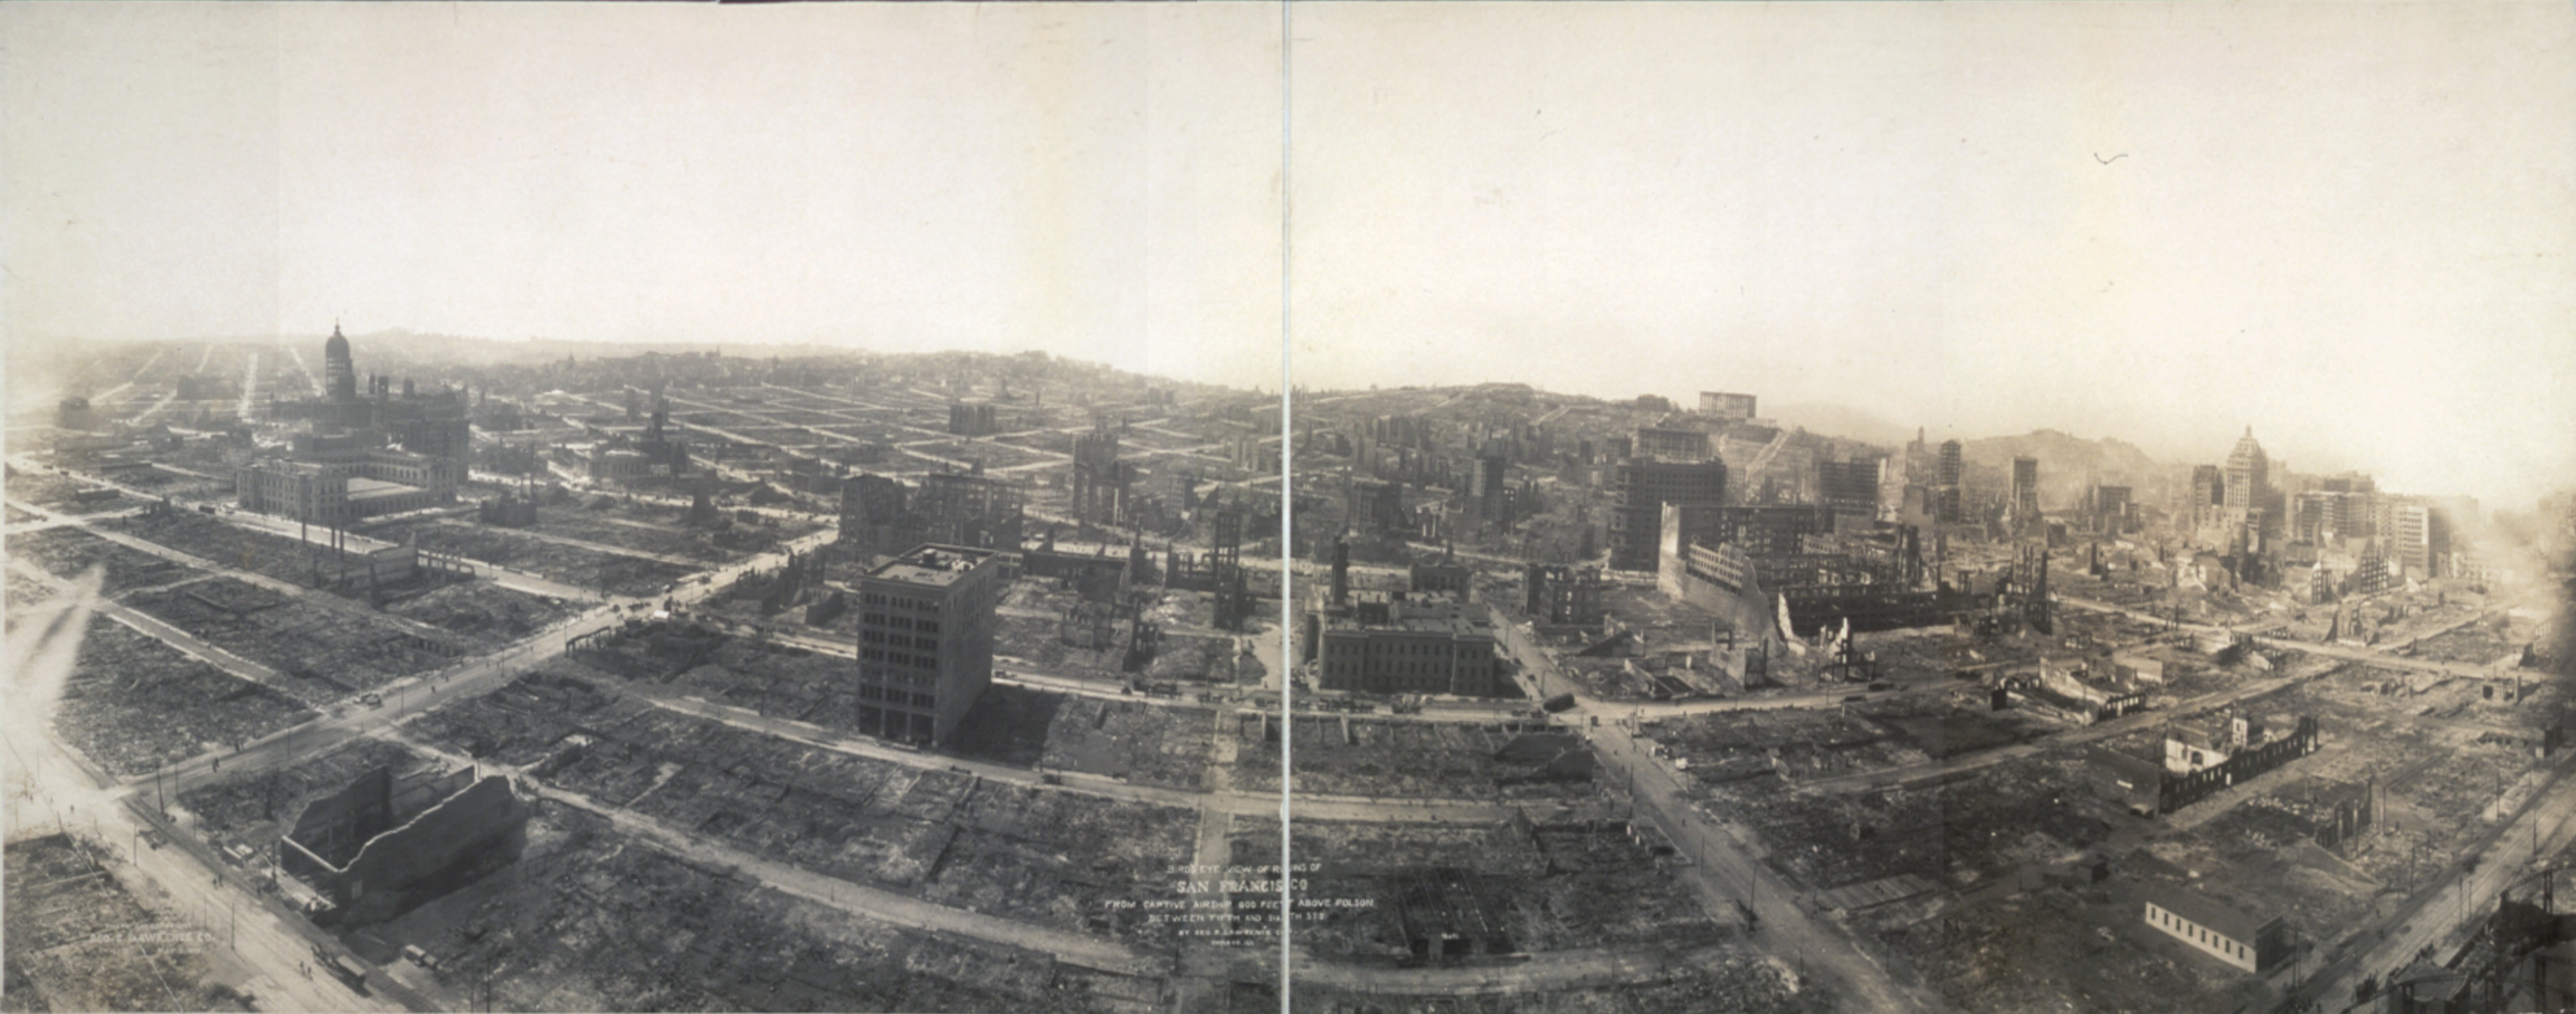
\includegraphics{figs/introduction/san_francisco_kitecamera.jpg}
	\caption{Photograph of San Francisco after the 1906 earthquake, taken from a camera held by seven kites. }
    \label{fig:san_francisco_kite}
\end{figure}

Satellite imaging, as known today, was first possible by the ideation of Konstantín Tsiolkovsky about rocketry to explore space, published under the title \textit{Exploring Space using jet propulsion devices}. This idea led to the first successful launch of the Sputnik satellite in 1957 and the development of Earth-orbiting satellites aimed at atmospherical monitoring. The Television and Infrared Observation Satellite (\acrshort{tiros}) was made operational in 1960 and integrated a small infrared system and a narrow-angle camera capturing data in the visible wavelengths. In 1978, a breakthrough change in satellites and coupled sensors came with \acrshort{tiros}-N (N for new). This spacecraft integrated a very high-resolution radiometer with 1 \si{\kilo\meter} footprint and four channels (visible, near-infrared, midrange-infrared and thermal infrared). Nowadays, an advanced version of these satellites is still operative under the name of \acrshort{avhrr} (Advanced Very High-Resolution Radiometer) with a similar footprint, though it captures six channels instead of four \cite{national_oceanic_and_atmospheric_administration_avhrr3_nodate}.   

\marginnote[.1cm]{An extensive repository of recent satellite missions can be found in the Earth Observation Portal, maintained by the European Space Agency \cite{earth_observation_portal_earth_nodate}.} 
From currently operative satellite programs, Landsat provides the largest collection of continuously acquired \acrshort{rs} data. It was first tested as part of NASA's NIMBUS program and there are currently two active satellites, Landsat 8 and Landsat 9, while the other seven have been terminated or planned to be decommissioned (Landsat 7). The payload of Landsat 9 consists of two instruments: Operational Land Imager (\acrshort{oli2}) and Thermal Infrared Sensor (\acrshort{tirs2}). A total of 11 bands and 740 scenes are collected every day, including red, blue, green, near-infrared, shortwave infrared, thermal, panchromatic, coastal and cirrus bands, ranging from a resolution of 15 \si{\meter} to 100 \si{\meter}. Other notable satellite programs are the China–Brazil Earth Resources Satellite (\acrshort{cbers}) and the Copernicus programme financed by the European Commission. The acrshort{cbers}-04A satellite is equipped with three imaging tools capturing five different spectrum intervals with a spatial resolution of 2-55 \si{\meter} \cite{instituto_nacional_de_pesquisas_espaciais_inpecbers_2019}. On the other hand, the Sentinel-2 mission acquires 13 bands in the visible, shortwave and near-infrared spectrum (see Figure \ref{fig:sentinel2}) with a spatial resolution ranging from 10 \si{\meter} to 60 \si{\meter} \cite{european_environment_agency_eu_2017}. Its cycle to revisit the same Earth's location is ten days, in comparison with the 16 days needed by Landsat 9 or 31 days from acrshort{cbers}-04A.

\begin{marginfigure}[-1.5cm]
	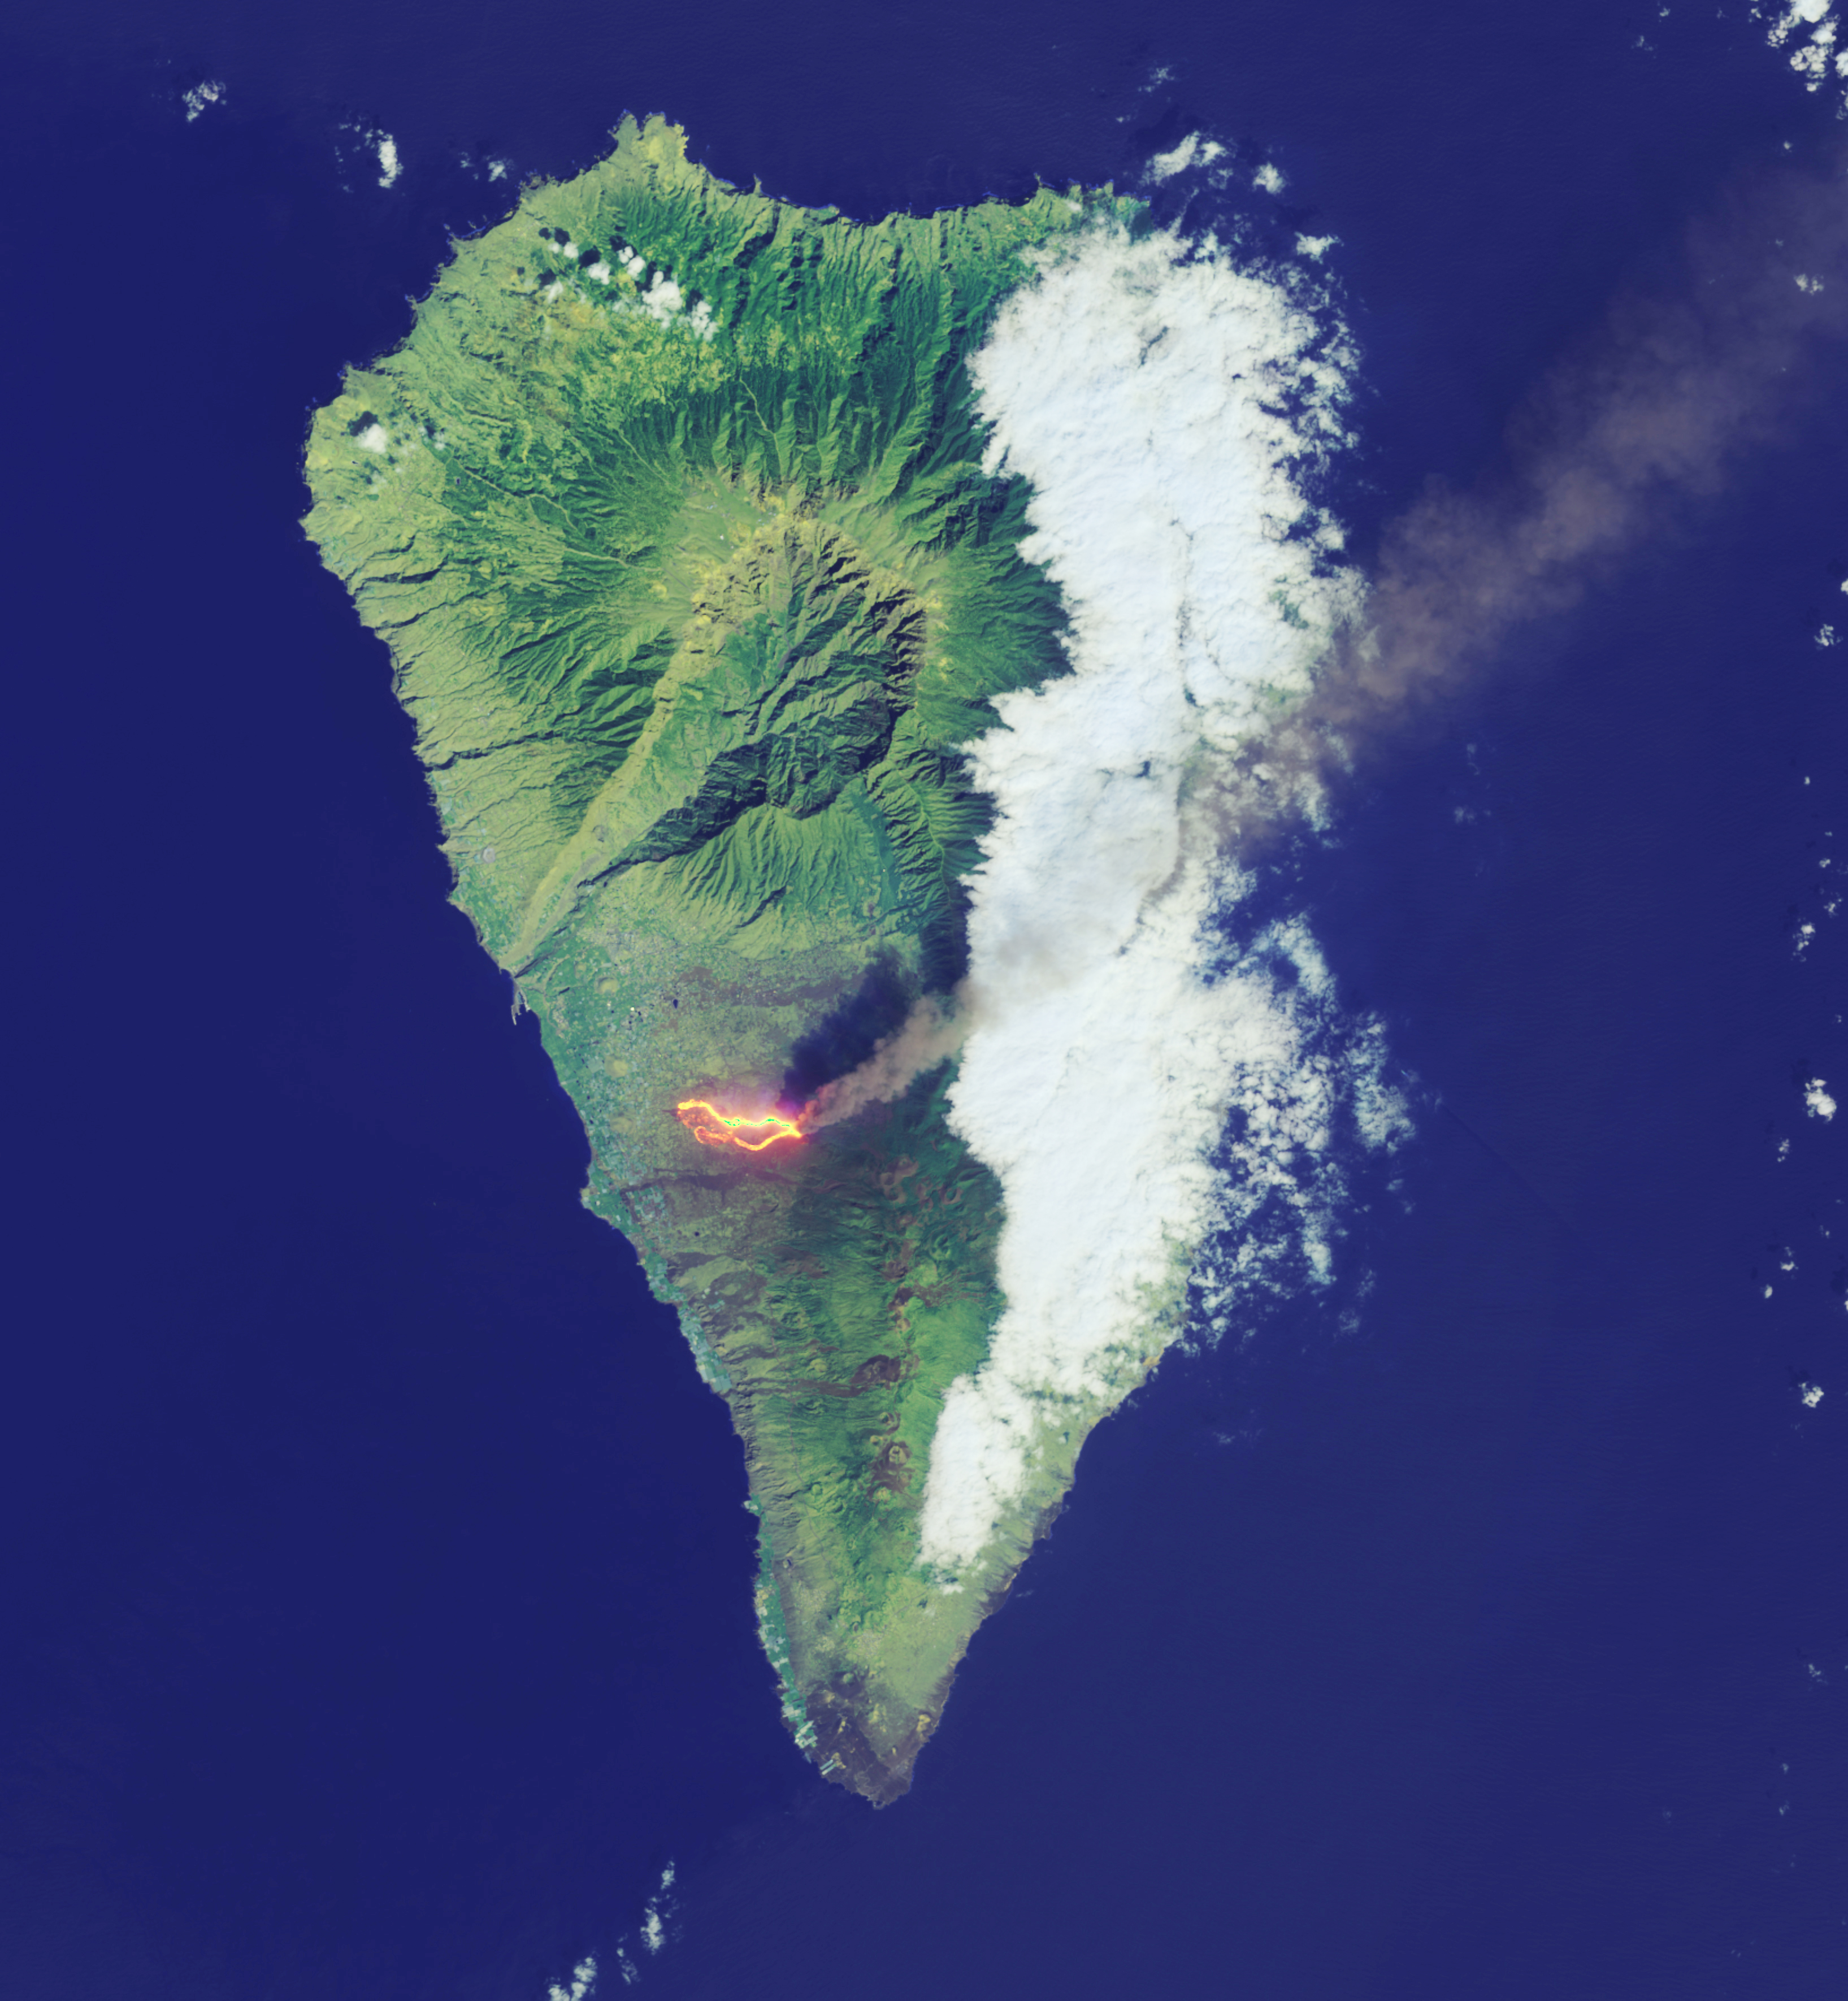
\includegraphics{figs/introduction/landsat8_lapalma.jpg}
	\caption{Cumbre Vieja volcano eruption observed from Landsat-8 \cite{nasa_earth_observatory_lava_2021}.}
	\label{fig:la_palma_landsat8}
\end{marginfigure}

\begin{figure}[!ht]
	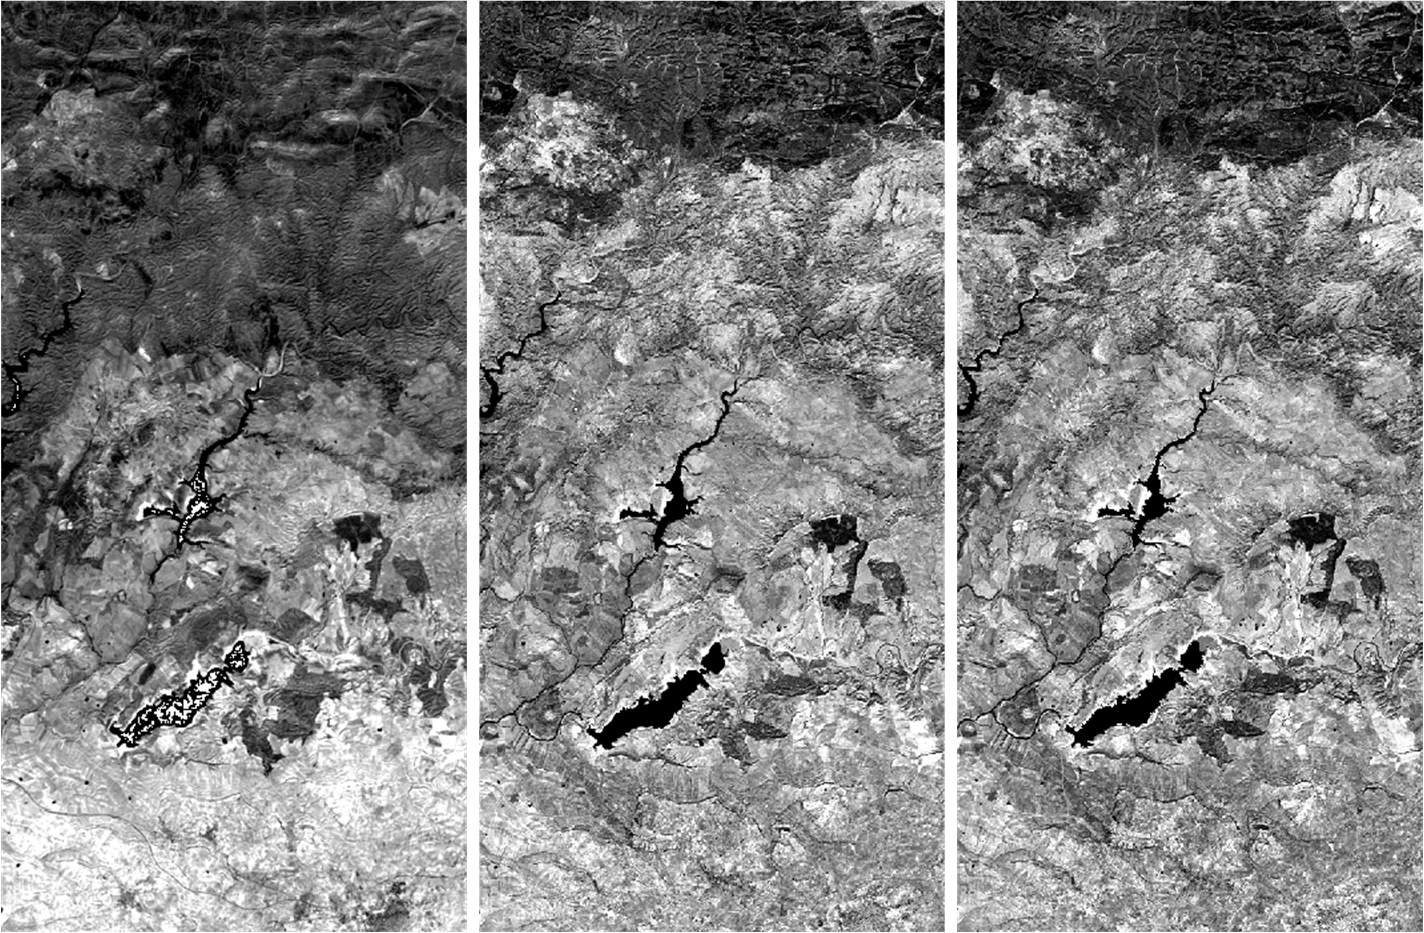
\includegraphics{figs/introduction/sentinel2_bands.png}
	\caption{Three shortwave infrared bands acquired by Sentinel-2 (band 9, 935-955 \si{\micro\meter}, band 11, 1567-1658 \si{\micro\meter}, and band 12, 2114-2889 \si{\micro\meter}). }
    \label{fig:sentinel2}
\end{figure}

Therefore, satellite imaging is better suited for the monitoring of changes over large areas using time series spanned over months and years. These data help to understand the dynamics of human and nature interaction as well as the impact of natural phenomena (Figure \ref{fig:la_palma_landsat8}). Some applications of the large collections of available satellite data are the analysis of land use, deforestation, land changes and urban settlements \cite{asokan_change_2019}. Nevertheless, the spatial resolution and revisit period of non-commercial satellite programmes harden their applicability to fine-grained monitoring tasks. The level of detail (\acrshort{lod}) of these tasks can refer to spatial resolution, temporal resolution or both, which are the main limitations of satellite imaging besides their cost. In spite of the described drawbacks, the use of satellite imagery is on the rise due to the steady reduction of Ground Sampling Distance (\acrshort{gsd}) and low periods for revisiting the same points. For instance, the commercial satellite Pléiades Neo (VHR-2020) from Airbus Defense \& Space \cite{airbus_pleiades_2021} is able to daily acquire seven bands with a \acrshort{gsd} of up to 30 \si{\centi\meter} for panchromatic images. Even for governmental missions, the repeat cycle is typically reduced as several twin missions could be active at the same moment with similar instruments and orbits. Accordingly, the offset in Landsat-8 and Landsat-9 trajectories allows acquiring data from the same point every 8 days \cite{masek_landsat_2020}. Still, spaceborne platforms are the most expensive Remote sensing technology by a huge lead.

Figure \ref{fig:scopus_search_platforms} depicts the amount of research devoted to each remote sensing platform. The Scopus searches were the following: $(p_1 \lor p_2 ... \lor p_n) \land (\textit{remote} \hspace{1mm} \land \hspace{1mm} \textit{sensing})$, with $p_i$ being one of platforms depicted in the legend. 

\begin{figure}[!ht]
	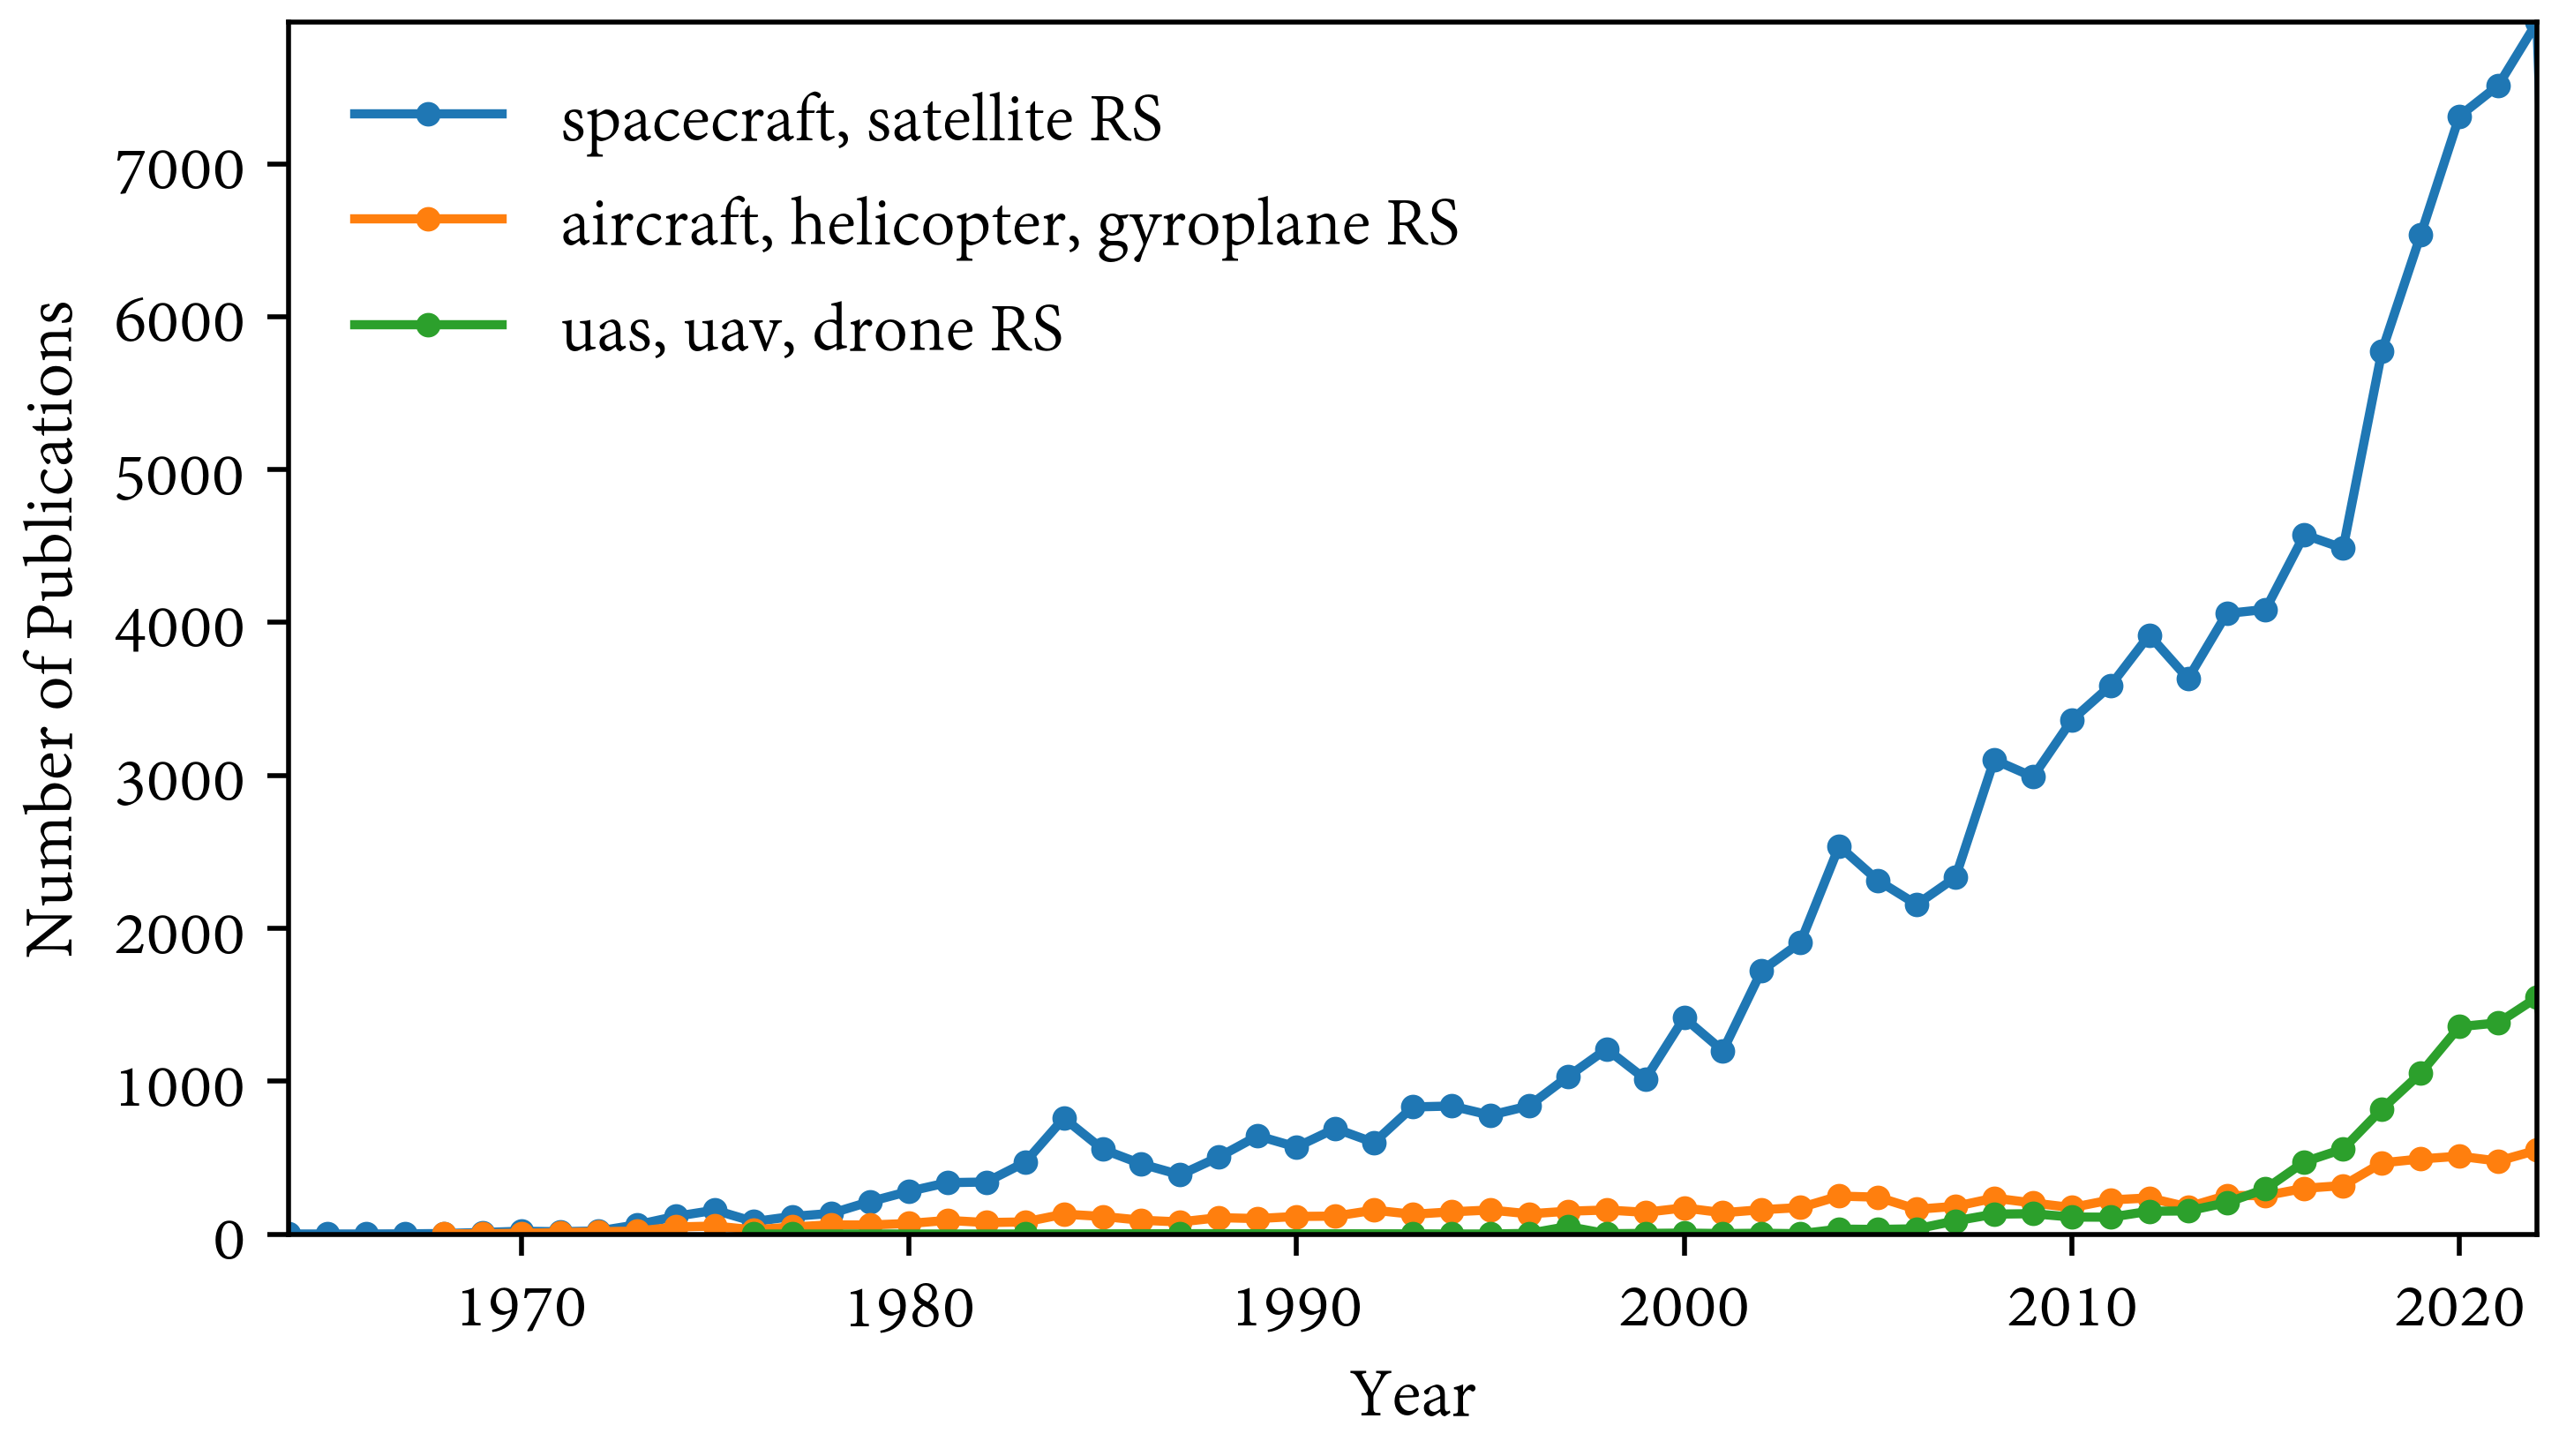
\includegraphics[width=\linewidth]{figs/introduction/platform_timeline.png}
	\caption{Number of manuscripts related to different \acrshort{rs} platforms. }
    \label{fig:scopus_search_platforms}
\end{figure}

However, it was until recently that satellite resolution was restricted by governments. These restrictions as well as the described limitations led to the use of alternative platforms. Besides satellites, airborne (fixed-wing and helicopters), Unmanned Aerial Systems (\acrshort{uas}) (Figure \ref{fig:dji300}) and other land platforms (mobile and static proximal-sensing) are the most frequent \cite{lillesand_remote_2015}. The choice of any of them always involves trade-offs concerning manoeuvrability, land coverage, repeat coverage, spatial resolution, spatial accuracy, cost or field of view (\acrshort{fov}) \cite{toth_remote_2016}. However, \acrshort{uas} have been gaining interest in the last decade as they transitioned from military tools in the early 2000s to easy-to-deploy, small and low-cost systems, thus widening their applicability to civilian activities and research. These platforms range from hand-sized to large aircraft that can be either controlled by human intervention or be partially, even fully, autonomous. Figure \ref{fig:dji300} shows a standard \acrshort{uas} designed by DJI which can carry up to 2.7 \si{\kilo\gram}, with a size of $501 \times 403 \times 252$ \si{\milli\meter}.
\begin{marginfigure}[-3cm]
	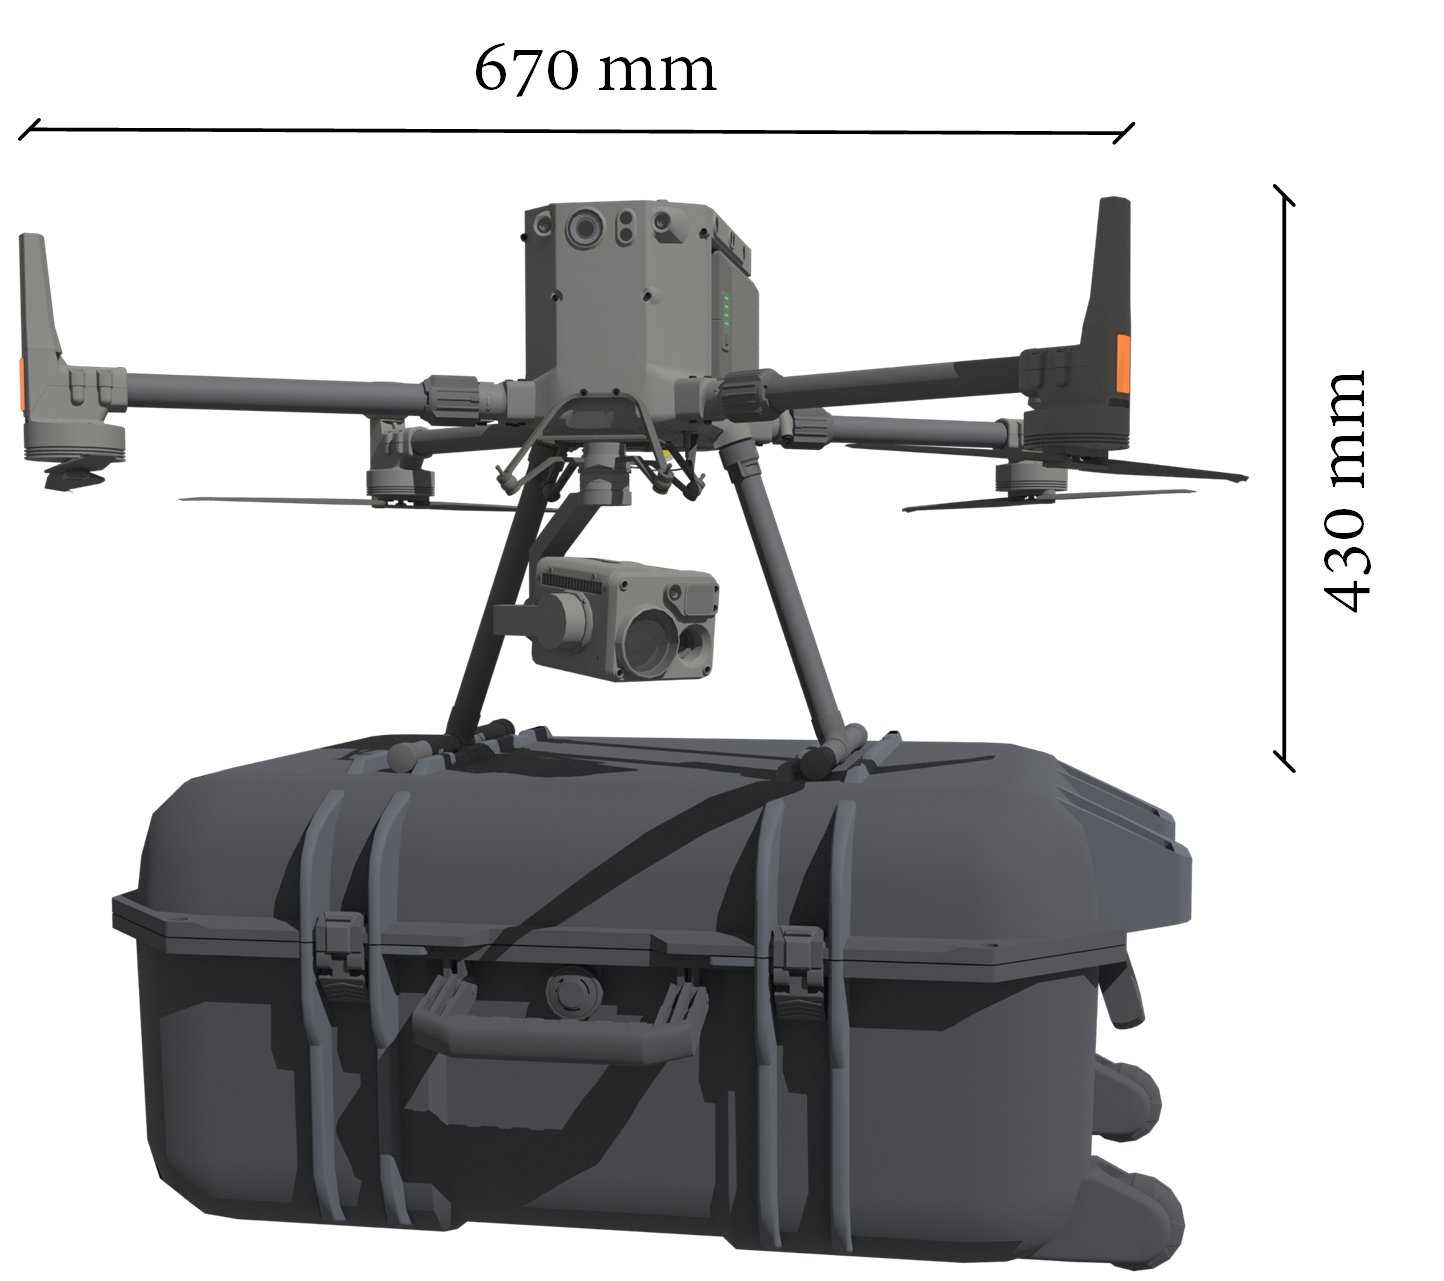
\includegraphics{figs/introduction/dji300.png}
	\caption{Quadcopter Matrice 300 RTK coupled with a dual RGB-thermal sensor (Zenmuse H20T). }
	\label{fig:dji300}
\end{marginfigure}

\begin{figure}[!ht]
	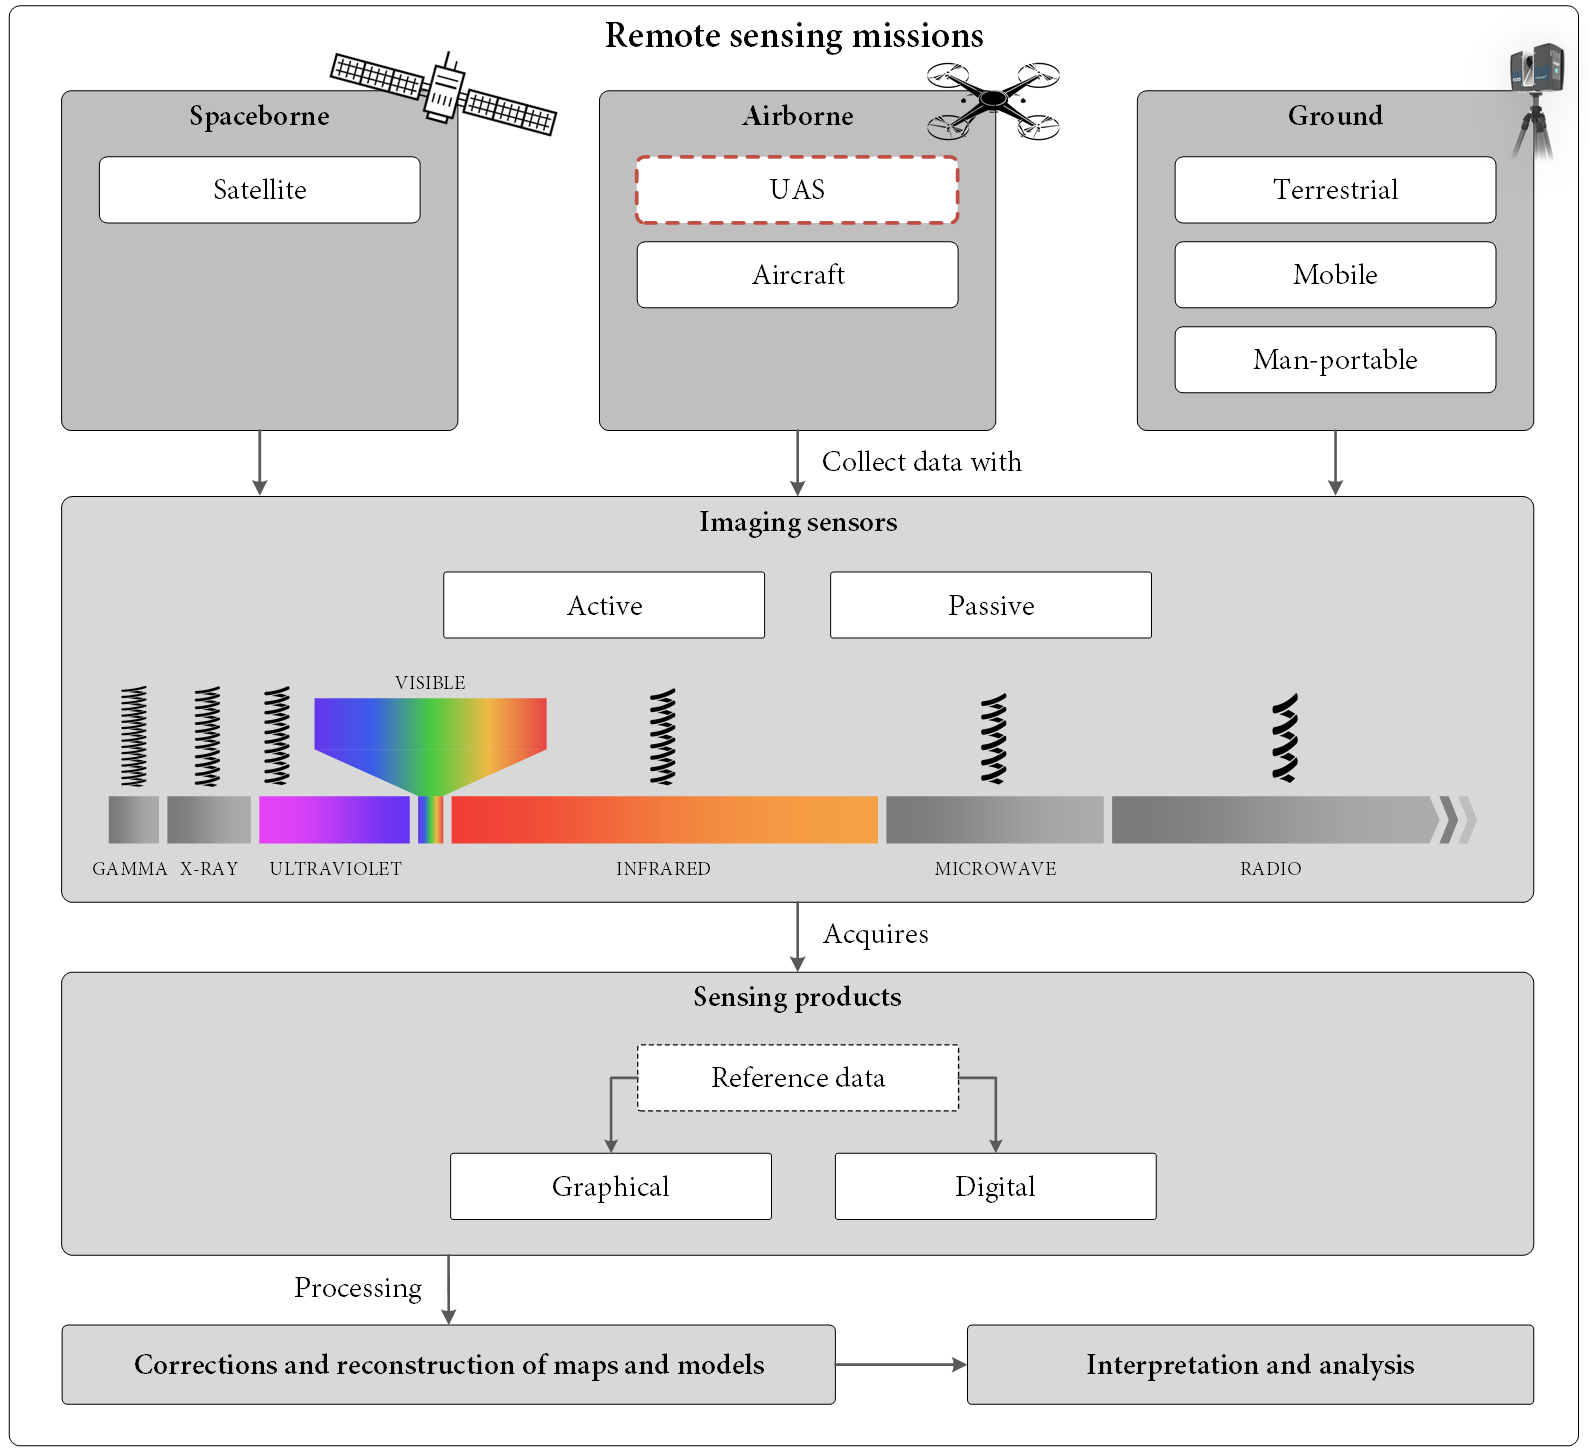
\includegraphics{figs/introduction/introduction_scheme.png}
	\caption{Overall procedure to acquire data with remote sensing platforms and sensors. Firstly, sensors are coupled on spaceborne, airborne and terrestrial vehicles or operated by humans, either by carrying them as a backpack or in hand. Then, sensor products can be grouped into graphical and numerical results, though most of them produce both kinds of data. Finally, the sensing products are processed and interpreted to provide users with valuable analyses. }
    \label{fig:introduction_scheme}
\end{figure}

The most frequent components of remote sensing \acrshort{uas} are imaging sensors as well as navigation and communication systems. The latter allows the operator to manoeuvre the platform within a communication range and transfer data in a bidirectional stream. Regardless of the navigating mission, either manual or waypoint-based, Global Positioning System (\acrshort{gps}) and Inertial Measurement Unit (\acrshort{imu}) sensors are used to calculate and record the craft's position, orientation and movement. These components are especially relevant to perform accurate flight missions, and their precision is generally described by means of vertical and horizontal error in meters (\si{\meter}). In this regard, the most recent \acrshort{uas} series from DJI achieve vertical and horizontal errors of up to 1 \si{\meter} using Real-time Kinematic (\acrshort{rtk}) positioning rather than \acrshort{gps}. As one would expect, \acrshort{uas} with lightweight and high-performance navigation sensors are more cost prohibitive than those with coarse navigation.    

In terms of safety regulations, the term \acrshort{uas} does not only refer to the vehicle but also to the coupled sensors, which are following introduced. Sensors typically coupled on aircraft vary according to the platform's flight altitude and cruising speed as well as application requirements. Fixed and rotating wing \acrshort{uas} solutions are considerably more limited in flying height and speed than other airborne vehicles, including helicopters and gyroplanes. Apart from platform limitations, the flight altitude may be limited by \acrshort{uas} regulations to avoid entering the domain of other airspace vehicles. Therefore, sensors and missions that require lower speed, lower flight altitude, and thus higher precision, are especially convenient for \acrshort{uas}. A widespread example of this is the monitoring of transmission lines, which happens to have a very thin structure and therefore require slower mapping. In comparison, other technologies such as Interferometric synthetic aperture radar (\acrshort{insar}) have been mainly applied to spaceborne missions to track changes on the Earth's surface.
\marginnote[-3cm]{The operability of unmanned aircraft over the Single European Sky airspace is controlled in the European Union by regulation 2019/947. Among other rules, the maximum flight altitude is established as 120 \si{\meter} over the Earth's surface unless an obstacle is overflown.} 

Therefore, \acrshort{uas} represent a cost-efficient tool for acquiring high-resolution data. The most common sensors mounted on UAS are cameras and \acrshort{lidar} (Light Detection and Ranging) sensors, with the first comprising a large number of imaging devices. Similarly, these groups also lead to the distinction between passive and active sensors. While the second has both transmitter and receiver components, the first is only aimed at capturing incoming radiance from the scene surfaces. However, the acquisition of multiple high-resolution datasets poses several advantages and drawbacks. 

\marginnote[.1cm]{The digitization of assets, processes and systems is greatly helped by reconstructions from sensor data. These allow connecting virtual and physical replicas through a data stream, thus shaping the fundamentals of \textbf{Digital twins}.}
Firstly, observations from multiple sensors can be interpreted as different features that complete a knowledge-based system, with each one providing information within a wavelength range. Furthermore, most of the algorithms aimed at analyzing and drawing conclusions from sensor data benefit from the use of complementary features. The contribution of each one in the extracted conclusions can be adjusted through weights that determine how important are these for the analysis. Unless a large number of features are used, which can lead to the curse of dimensionality problem, it is safe to say that the greater number of features, the better. On the other hand, high-resolution data help to generate precise models that are easier to analyze and visualize by human operators. Denser data also involves denser geometry and reconstructions, thus omitting fewer details of target surfaces and easing the construction of digital models that emulate the Earth's scenarios and processes. 

Different layers of information are ideally noise-free and represented under the same coordinate system. In the reality, navigation sensors present small positioning errors that harden the fusion of several layers of information. Despite being small, these are reported as shifts, rotation and scale variations among different sensor data. Furthermore, environmental conditions such as atmospheric composition, wind, temperature or solar radiation can vary from one flight to another and so do the acquired data, even under similar flight plans. These changes not only affect observations performed in a short period of time with different sensors but also time series acquired with previously used tools. Although tedious, variations concerning positioning and orientation errors can be diminished by including reference points measured with sensors of higher precision in easily recognizable image features. Other shortcomings are the noise induced by faulty device detectors, especially for active sensors, unwanted atmospheric particles and surfaces whose bouncing behaviour leads to unreal geometry. Therefore, a system capable of accurately fusing the outcome of every sensor integrated with a \acrshort{uas} is necessary to facilitate the later processing stages and provide reliable conclusions. 

Sensing products are typically transformed into other data representations that are not provided by the sensor. Accordingly, individual images are not sufficient to interpret the scenario in some contexts. A complete vision of it can be provided by joining images, thus resulting in 2D maps and 3D points calculated by estimating the camera pose and finding features in common among several images. During these transformations, estimated radiometric and geometric properties can be affected by precision loss on the interpolation, and therefore, a comparison can be established with other reliable data sources. For instance, \acrshort{lidar} is known to generate accurate point clouds that can be used as the reference to compare the quality of point clouds reconstructed from imagery. Similarly, images can serve as reference data for measuring radiometric dissimilarity.   

On the other hand, large volumes of data are also harder to operate in terms of computing, storage and visualization. Thousands of images or millions of points can be hardly operated in commodity hardware due to the required storage and computing capabilities. However, current trends in informatics have favoured the proliferation of personal and professional computers with large storage capacity, more efficient access to data and great multi-threading capabilities. The latter can be performed over the Central Processing Unit (\acrshort{cpu}), whose trend is to increase the number of cores, and the Graphic Processing Unit (\acrshort{gpu}), composed of millions of units that can massively solve small tasks and cooperate among small thread groups. Chapter \ref{sec:fundamentals_rs} delves into the most common data formats in \acrshort{rs}; at this moment, it is enough to think of data as large volumes of digital numbers (\acrshort{dn}). Despite large storage being inexpensive nowadays, challenges such as the partial retrieval of information remain, especially for interactive applications with high data throughput \cite{bejar-martos_strategies_2022, ogayar-anguita_nested_2023}. 

\begin{marginfigure}[.5cm]
	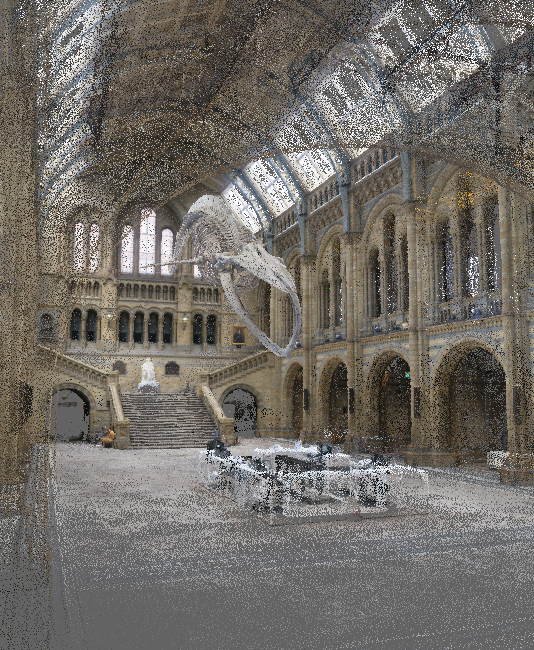
\includegraphics{figs/introduction/hintze.png}
	\caption{Point cloud with 2.4M points reconstructed using 900 photos at the Hintze Hall (Model uploaded by \textit{Thomas Flynn} in \textit{Sketchfab}).  }
	\label{fig:hintze_hall}
\end{marginfigure}
Another drawback in real-time applications is the visualization of these large volumes of data. Traditional rendering pipelines are built as a set of static stages, where the model geometry and topology are iteratively transformed into pixels. The colours of these come from the shading of one or multiple light sources over the textures of a surface, using a discretization of the formulae that describe light interaction. Unlike synthetic models designed by human operators, most sensor data are shaded according to the recorded wavelengths. Thus, alternative pipelines are needed to visualize these data. According to the \acrshort{gpu} architecture, the data can be sorted and organized in data structures in pursuit of workload balancing and geometry simplifications that help to trick user perception. These requirements are even stricter for Virtual Reality (\acrshort{vr}) devices that render every scenario at least once for each eye, and even more whether other rendering techniques are included, e.g., shadow mapping.  

Previous methods are simply a procedure that allows extracting text-based or visual clues that help in the recognition of weaknesses and failures in processes. Accordingly, the last step is to classify, segment and recognize features from input data to optimize future operations. The main contributions of \acrshort{rs} techniques in Precision Agriculture (\acrshort{pa}) are yield estimation, crop-type inventory, measuring of water content and Leaf Area Index (\acrshort{lai}), control of diseases and insects as well as moisture, changes, growth, stress and drought monitoring, among other risk factors such as snow or fire \cite{huang_agricultural_2018}. These monitoring tasks are intended to maximize profitability and minimize waste and pollution. 
\marginnote[-3cm]{This dissertation has Precision Agriculture (\acrshort{pa}) as its main research field and therefore, the data analysis has been narrowed to 1) segment crops into ground and vegetation, and 2) phenotyping of a large number of plant varieties in a non-destructive way.}

A significant number of datasets have been published with the steadily increasing importance of imagery classification using Machine Learning (\acrshort{ml}) and Deep Learning (\acrshort{dl}) methods from Artificial Intelligence (\acrshort{ai}). Thus, the analysis stage is nowadays easier than ever to implement using large datasets over which \acrshort{ai} algorithms train and learn. However, most of the large \acrshort{rs} image collections are based on spaceborne sensors capturing a wide range of scenarios, while they barely address datasets that may be helpful in \acrshort{pa}. Another challenge arises from the labelling of large datasets, as it must be performed by unsupervised algorithms, which transform and extract relevant features, or human operators \cite{li_image_2021, basu_deepsat_2015}. None of these methods is perfect and thus can result in spurious labelling data that can mislead the learning algorithms. Furthermore, manual tagging is typically done over visible bands, which are easier to interpret for humans, and therefore, only a few datasets include bands further than \acrshort{rgb}. In this regard, hyperspectral sensors mitigate the latter problem as they co-acquire a large number of bands from which we can extract a false colour image that imitates an RGB product.

Although some notable datasets exist for \acrshort{rs}, as well as a wide variety of sensors and spectral bands, these may not be valid for case studies that fall out of state-of-the-art trends. It is possible to conduct many surveys and create datasets on our own. However, it is incredibly time-consuming to acquire, process and extract features, including labels, as these manual tasks require computational resources and human operators. At least partially, data from sensors could be synthetically generated by emulating the sensor mechanism. The main advantage is that data acquired from a virtual sensor are linked to digital models without uncertainty. Likewise, digital models are augmented with features that could be directly transferred to the sensing results. The most frequently simulated sensors are Radar and \acrshort{lidar} systems, though synthetic images have also been recently generated with the rise of \acrshort{dl} approaches capable of generating new data.  

\section{Aims and objectives}

According to previously presented challenges, the overall aim of this dissertation is to contribute to some of the stages presented in Figure \ref{fig:introduction_scheme}. A significant number of challenges have already been briefly reviewed, including the collection of datasets from multiple sensors, difficulties in the correction and fusion of these, the generation of products with larger dimensionality (e.g., 2D $\rightarrow$ 3D) or the analysis of final products. According to this, the objectives of this work are the following:
\begin{itemize}
    \item The correction and processing of data as collected by airborne surveys. Rather than a single front, this objective involves studying how can be every data source corrected, including geometrical and radiometric distortions. The first must be solved in most cases, since it enables the later fusion of data, whereas the latter depends on whether the radiance is further analyzed or not.
    \item The matching of images collected by different sensors, thus overcoming differences concerning 1) triggering timestamps, 2) optical aberrations, 3) optical systems and 4) wavelength intervals. The image matching ought to work over images with notable intensity dissimilarity to obtain reliable transformations that allow projecting one data source into another. 
    \item The efficient generation of large and dense 3D point clouds from multiple data sources without geometric inaccuracies. The proposed pipeline ought to tackle most of the drawbacks of traditional photogrammetry. In addition, this is a time-consuming task that is further stressed by including multiple data sources; hence, it must be addressed using accelerated computing.
    \marginnote[.35cm]{Despite previous datasets covering a wide part of the spectrum, these were projected to a 3D baseline point cloud, generated with photogrammetry. Image-based reconstructions are less reliable than other optical sensing products, such as \acrshort{lidar}, which directly acquires 3D data from collided surfaces. However, it is considerably more cost prohibitive than most of the revised optical imaging sensors.}
    \item To emulate \acrshort{lidar} sensors over 3D synthetic scenarios. Nonetheless, this is also a time-consuming task that is especially tough to model in terms of returned intensity. The efficient generation of large labelled \acrshort{lidar} datasets must be addressed, again, using accelerating computing, and modelling the surfaces' properties.
    \item To demonstrate the applicability of previous results. Though not exhaustive, this objective involves detecting anomalies, segmenting some items apart from others or phenotyping a large number of vegetation varieties. It can be either performed with traditional geometry-based techniques as well as using \acrshort{ai} algorithms.
\end{itemize}

\section{Organization}

This dissertation comprises six different parts which are following detailed:

\newcommand{\partTabSize}{3mm}

\small \noindent \textbf{\textls[30]{PART I}} \normalsize\hspace{\partTabSize} This part includes the current chapter. A shallow introduction to \acrshort{rs} is presented together with the main challenges concerning data fusion. Then, the fundamentals of this dissertation are presented in Chapter \ref{sec:fundamentals_rs}, and later, a review of the state-of-the-art is given in Chapter \ref{sec:fundamentals_rs} to introduce previous work on the fusion and simulation of UAV-based data.

\small \noindent \textbf{\textls[30]{PART II}} \normalsize\hspace{\partTabSize} Here, the fundamentals of our methods are presented, including which kind of sensors and data are available. The correction and the image fusion algorithms are isolated in Chapter \nameref{sec:image_fusion}. In summary, this part comprises the materials and methods that are shared among most of this dissertation's chapters.

\small \noindent \textbf{\textls[30]{PART III}} \normalsize\hspace{\partTabSize} This part explains the generation of 3D point clouds consisting of multiple layers: visible, infrared, multispectral and hyperspectral data. The visible colour is presented as the baseline 3D point cloud that is enhanced with the rest of the datasets. First, thermographic imagery is fused with \acrshort{rgb} data to propose an efficient projection in the \acrshort{gpu}, the so-called \acrshort{gpu}. This procedure is following applied to multispectral data, despite this being significantly more time-consuming and intricate since the latter comprises four spectral bands. Then, a hyperspectral point cloud is generated following a different pipeline, yet accelerated, that fits the conditions on which these data were acquired.  

\small \noindent \textbf{\textls[30]{PART IV}} \normalsize\hspace{\partTabSize} Once available data is corrected and fused, those data sources not available are simulated using detailed synthetic scenarios that are rapidly labelled with semantic tags. Simulations are aimed at modelling products similar to those collected by real sensors, including their geometrical properties. The fundamentals of \acrshort{lidar} simulations are reviewed in Chapter \ref{sec:lidar_simulation}, whereas radiance properties require further considerations which are detailed in Chapter \ref{sec:lidar_intensity}. Then, these simulations are used to assist in the scanning of indoor scenarios such as buildings in Chapter \ref{sec:lidar_optimization}.

\small \noindent \textbf{\textls[30]{PART V}} \normalsize\hspace{\partTabSize} This part shows multiple applications of the collected data and the derived results, including the simulated \acrshort{lidar} point clouds, reconstructed thermal point clouds and hyperspectral swaths. The firsts are applied to the detection of thermal anomalies that may be linked to buried remains at an archaeological site. Hyperspectral swaths are, on the other hand, corrected and processed for the classification of red and white grapevine varieties using Deep Learning.

\small \noindent \textbf{\textls[30]{PART VI}} \normalsize\hspace{\partTabSize} Chapter \ref{sec:conclusions} concludes this dissertation by highlighting the main contributions and pointing out future work.